\documentclass[aspectratio=169]{beamer}

\mode<presentation>

\usepackage[utf8]{inputenc}
\usepackage[T1]{fontenc}	%makes å,ä,ö etc. proper symbols
\usepackage{amsmath}
\usepackage{graphicx}
\usepackage{xcolor}
\usepackage{listings}
\usepackage{multicol}
\usepackage{hyperref}
\usepackage[swedish]{babel}

\definecolor{LundaGroen}{RGB}{00,68,71}
\definecolor{StabilaLila}{RGB}{85,19,78}
\definecolor{VarmOrange}{RGB}{237,104,63}

\definecolor{MagnoliaRosa}{RGB}{251,214,209}
\definecolor{LundaHimmel}{RGB}{204,225,225}
\definecolor{LundaLjus}{RGB}{255,242,191}

\usefonttheme{serif}
\usetheme{malmoe}
\setbeamercolor{palette primary}{bg=LundaHimmel, fg=StabilaLila}
\setbeamercolor{palette quaternary}{bg=LundaGroen, fg=MagnoliaRosa}
\setbeamercolor{background canvas}{bg=LundaLjus}
\setbeamercolor{structure}{fg=LundaGroen}

\usepackage[many]{tcolorbox}

\newtcolorbox{cross}{blank,breakable,parbox=false,
  overlay={\draw[red,line width=5pt] (interior.south west)--(interior.north east);
    \draw[red,line width=5pt] (interior.north west)--(interior.south east);}}



\lstset{language=Python} 
\lstset{%language=[LaTeX]Tex,%C++,
    morekeywords={PassOptionsToPackage,selectlanguage,True,False},
    keywordstyle=\color{blue},%\bfseries,
    basicstyle=\small\ttfamily,
    %identifierstyle=\color{NavyBlue},
    commentstyle=\color{red}\ttfamily,
    stringstyle=\color{VarmOrange},
    numbers=left,%
    numberstyle=\scriptsize,%\tiny
    stepnumber=1,
    numbersep=8pt,
    showstringspaces=false,
    breaklines=true,
    %frameround=ftff,
    frame=single,
    belowcaptionskip=.75\baselineskip,
	tabsize=4,
	backgroundcolor=\color{white}
    %frame=L
}


\begin{document}

\lstset{literate=
  {á}{{\'a}}1 {é}{{\'e}}1 {í}{{\'i}}1 {ó}{{\'o}}1 {ú}{{\'u}}1
  {Á}{{\'A}}1 {É}{{\'E}}1 {Í}{{\'I}}1 {Ó}{{\'O}}1 {Ú}{{\'U}}1
  {à}{{\`a}}1 {è}{{\`e}}1 {ì}{{\`i}}1 {ò}{{\`o}}1 {ù}{{\`u}}1
  {À}{{\`A}}1 {È}{{\'E}}1 {Ì}{{\`I}}1 {Ò}{{\`O}}1 {Ù}{{\`U}}1
  {ä}{{\"a}}1 {ë}{{\"e}}1 {ï}{{\"i}}1 {ö}{{\"o}}1 {ü}{{\"u}}1
  {Ä}{{\"A}}1 {Ë}{{\"E}}1 {Ï}{{\"I}}1 {Ö}{{\"O}}1 {Ü}{{\"U}}1
  {â}{{\^a}}1 {ê}{{\^e}}1 {î}{{\^i}}1 {ô}{{\^o}}1 {û}{{\^u}}1
  {Â}{{\^A}}1 {Ê}{{\^E}}1 {Î}{{\^I}}1 {Ô}{{\^O}}1 {Û}{{\^U}}1
  {œ}{{\oe}}1 {Œ}{{\OE}}1 {æ}{{\ae}}1 {Æ}{{\AE}}1 {ß}{{\ss}}1
  {ű}{{\H{u}}}1 {Ű}{{\H{U}}}1 {ő}{{\H{o}}}1 {Ő}{{\H{O}}}1
  {ç}{{\c c}}1 {Ç}{{\c C}}1 {ø}{{\o}}1 {å}{{\r a}}1 {Å}{{\r A}}1
  {€}{{\euro}}1 {£}{{\pounds}}1 {«}{{\guillemotleft}}1
  {»}{{\guillemotright}}1 {ñ}{{\~n}}1 {Ñ}{{\~N}}1 {¿}{{?`}}1
}

\AtBeginSection[ ]
{
\begin{frame}{Innehåll}
    		\tableofcontents[currentsection]
\end{frame}
}

\title{if-satser}
\author{Programmering 1}
\date{2024/2025}

\maketitle


\section{else \& elif}

\subsection{else}

\begin{frame}[fragile]
	\frametitle{Annars}
	
	Senast pratade vi om ''om något gör något''. I dag lägger vi till ''annars gör detta''.
	
	\pause
	
	\begin{lstlisting}
svar = input("Är du glad?")
if svar == "ja":
	print("Vad bra :)")
if svar != "ja":
	print("Vad tråkigt :(")
	\end{lstlisting}
	
	\pause

	\begin{lstlisting}
svar = input("Är du glad?")
if svar == "ja":
	print("Vad bra :)")
else:
	print("Vad tråkigt :(")
	\end{lstlisting}

\end{frame}

\begin{frame}

	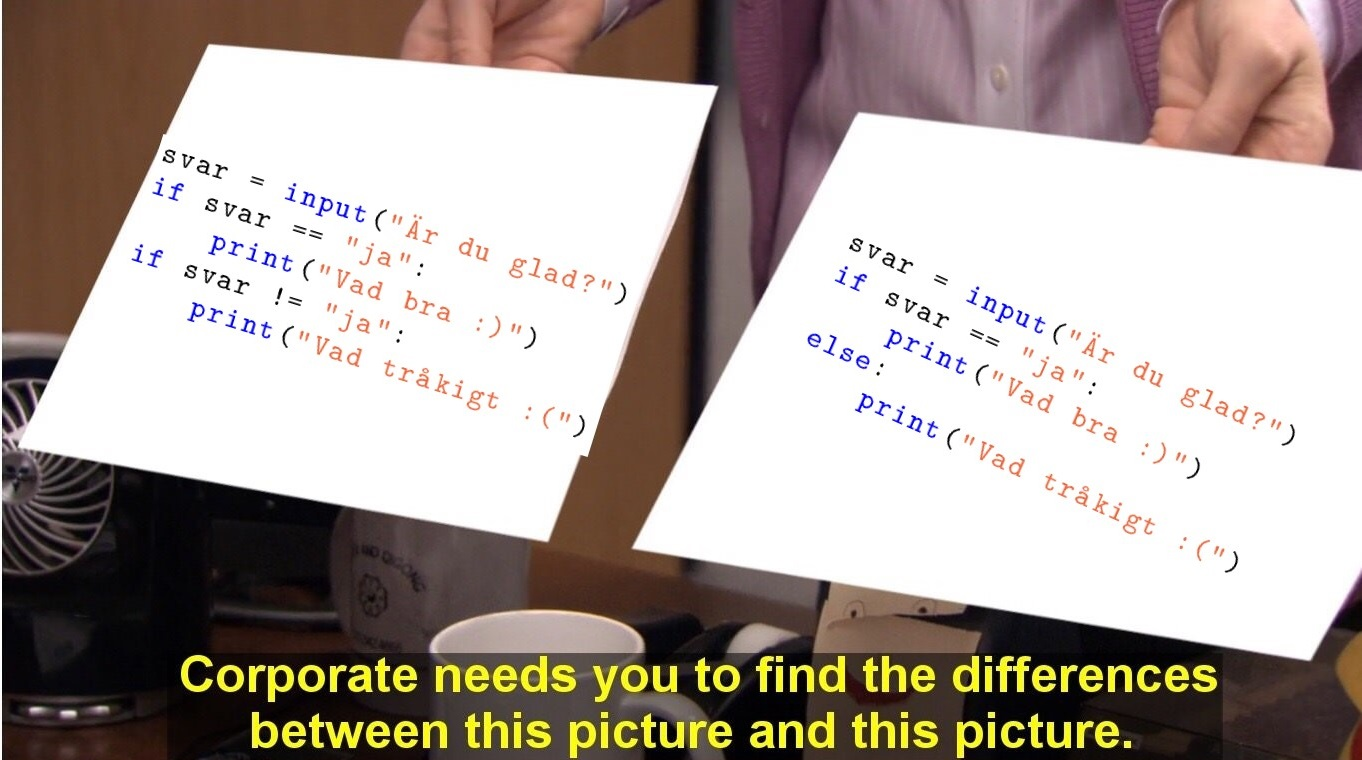
\includegraphics[width=\linewidth]{corporate1.jpg}

\end{frame}

\begin{frame}

	
\includegraphics[width=\linewidth]{corporate2.jpg}

\end{frame}

\begin{frame}[fragile]
	\frametitle{Annars}
	
	\begin{lstlisting}
tal = input("Skriv ett primtal mindre än tio: ")
tal = int(tal)

if tal == 2 or tal == 3 or tal == 5 or tal == 7:
	print("Rätt")
else:
	print("Fel")
	\end{lstlisting}
	
	\begin{itemize}
		\item \lstinline{else} är ett smidigt sätt att ta hand om alla fall som inte stämmer överens med ursprungsvillkoret.
		\item Avslutar man sin jämförelse med \lstinline{else} kan man vara säker på att koden kommer att gå in i något av blocken
	\end{itemize}


\end{frame}

\subsection{elif}

\begin{frame}[fragile]
	\frametitle{Annars om}
	
	\begin{lstlisting}
antal = input("Hur många Pokémon finns det?")
antal = int(antal)

if antal == 151:
    print("Kaaaaanske. Vi säger så.")
elif antal > 151:
    print("Du är nog yngre än mig")
else:
    print("Har du noll koll?")
	\end{lstlisting}
	
	Ett \lstinline{elif} villkor kollas bara om inget av villkoren tidigare har uppfyllts. 


\end{frame}

\begin{frame}[fragile]
	\frametitle{Exempel}

	Det är helt okej att villkorssatserna överlappar, Python kommer inte ge något felmeddelande. Men det är onödigt.
	
	\begin{lstlisting}
ålder = input("Hur gammal är du? ")
ålder = int(ålder)

if ålder >= 18:
    print("Nu är du myndig. Begå inga brott!")
elif ålder >= 65:
    print("Du är pensionär.")
else:
    print("Du röstade inte i det senaste riksdagsvalet.")
	\end{lstlisting}

	\pause
	
	Det här programmet kommer aldrig att skriva ut ''\texttt{Du är pensionär}'', eftersom den \lstinline{elif}-satsen bara kan vara sann om \lstinline{if}-satsen ovanför är sann. Och eftersom \lstinline{elif} står för ''\textbf{annars} om'' så inträffar den inte.

\end{frame}

\begin{frame}[fragile]
	\frametitle{Exempel}
	
	Om man vill att programmet ska markera om någon är pensionär kan man göra så här:
	
	\begin{lstlisting}
ålder = int(input("Hur gammal är du? "))

if ålder >= 18:
    print("Nu är du myndig. Begå inga brott!")
    if ålder >= 65:
        print("Du är pensionär.")
else:
    print("Du röstade inte i det senaste riksdagsvalet.")
	\end{lstlisting}
	
	Skriver man in att man är 70 år gammal nu så kommer programmet att spotta ut:
	
	\begin{lstlisting}
Nu är du myndig. Begå inga brott.
Du är pensionär.
	\end{lstlisting}

\end{frame}

\begin{frame}[fragile]
	\frametitle{If på if}
	
	\begin{lstlisting}
ålder = int(input("Hur gammal är du? "))

if ålder >= 18:
    print("Nu är du myndig. Begå inga brott!")
    if ålder >= 65:
        print("Du är pensionär.")
else:
    print("Du röstade inte i det senaste riksdagsvalet.")
	\end{lstlisting}
	
	Notera att den andra \lstinline{if}-satsen är indragen till samma nivå som raden ovanför. Det är även så att det sista meddelandet BARA skrivs ut om man svarar att man är under 18. Det syns tydligast på att \lstinline{else} har samma indenteringsnivå som \lstinline{if ålder >= 18:}

\end{frame}

\begin{frame}[fragile]
	\frametitle{If på if}
	
	\begin{lstlisting}
ålder = int(input("Hur gammal är du? "))

if ålder >= 18:
    print("Nu är du myndig. Begå inga brott!")
    if ålder >= 65:
        print("Du är pensionär.")
    else:
        print("Du är i arbetsför ålder.")
else:
    print("Du röstade inte i det senaste riksdagsvalet.")
	\end{lstlisting}
	
	Om man nu svarar att man är 20 år gammal svarar programmet så här:
	
	\begin{lstlisting}
Nu är du myndig. Begå inga brott!
Du är i arbetsför ålder.
	\end{lstlisting}

\end{frame}

\begin{frame}[fragile]
	\frametitle{Flera elif}

	Man kan ha hur många \lstinline{elif} efter varandra man vill:
	
	\begin{lstlisting}
ålder = int(input("Öh, din ålder? "))
if ålder == 0:
    print("Bebis")
elif ålder == 1:
    print("Fortfarande bebis")
elif ålder == 2:
    print("Så liten")
elif ålder == 3:
    print("Halvägs till", ålder*2)
elif ålder == 4:
    print("2 i kvadrat gammal. Grattis.")
	\end{lstlisting}
	
	Man behöver inte heller ha något \lstinline{else} alls.

\end{frame}

\section{Övningar}

\begin{frame}[fragile]
	\frametitle{Övningar}
	\framesubtitle{Blad 1}
	
	Utgå från filen \texttt{if-else.py} i Classroom.

	\begin{enumerate}
		\item Det finns en logisk bugg i raderna 12--15. Rätta till den.
		\item Skriv ett program som tar emot ett tal och skriver ut olika saker baserat på talet. Se filen \texttt{if-else.py} för meri nformation.
		\item Skriv ett program som kollar om ett ord är skrivet med bara versaler, gemener eller om det är blandat.
		\item Skriv ett program som tar emot ett årtal (efter 1753) och returnerar om det var ett skottår eller ej. Tänk på att år jämnt delbara med 100 inte är skottår, men att år delbara med 400 är fortfarande skottår. (1800 och 1900 ej skottår men 2000 och 2400 skottår.)
	\end{enumerate}

\end{frame}


\begin{frame}
	\frametitle{Övningar}
	\framesubtitle{Blad 2}
	
	\begin{enumerate}
		\setcounter{enumi}{4}
		\item Skriv ett program som tar emot ett tal och kollar om det är jämnt delbart med två
		\item Skriv ett program som tar emot ett tal och kollar hur många gånger det är delbart med två
		\item Följ instruktionerna i filen ''\texttt{fil med fel.py}''
	\end{enumerate}

\end{frame}


\end{document}